\documentclass[journal]{IEEEtran}

\usepackage{amsmath}
\usepackage{amssymb}
\usepackage{graphicx}
\usepackage{booktabs}
\usepackage{cite}
\usepackage{hyperref}
\usepackage{listings}
\usepackage{xcolor}
\usepackage[ruled,vlined,linesnumbered]{algorithm2e}

\definecolor{codegray}{rgb}{0.5,0.5,0.5}
\definecolor{backcolour}{rgb}{0.95,0.95,0.92}

\lstdefinelanguage{json}{
    basicstyle=\ttfamily\footnotesize,
    string=[s]{"}{"},
    stringstyle=\color{blue},
    comment=[l]{//},
    commentstyle=\color{codegray},
    morestring=[b]',
}

\lstset{
    backgroundcolor=\color{backcolour},   
    commentstyle=\color{codegray},
    basicstyle=\ttfamily\footnotesize,
    breakatwhitespace=false,         
    breaklines=true,                 
    captionpos=b,                    
    keepspaces=true,                 
    showspaces=false,                
    showstringspaces=false,
    showtabs=false,                  
    tabsize=2
}

\begin{document}

\title{Vertical Dual-Gate Trees: A Deterministic Approach to Traceability and Hallucination Mitigation in Requirements Engineering}

\author{
    \IEEEauthorblockN{Taher Awad, Ahmed Abdo Ahmed, Khalid Abdelsalam, and Ahmed Abdallah}
}

\maketitle

\begin{abstract}
The integration of Large Language Models (LLMs) into the software development life cycle has significantly accelerated automated code generation. However, in deep Requirements Engineering (RE) pipelines, these generative processes often suffer from severe hallucination and context loss, resulting in disconnected architectural artifacts and test cases. Multi-agent and unbounded Chain-of-Thought approaches face combinatorial token explosion and context-bleed issues. To solve this problem, we propose the ``Vertical Dual-Gate Tree,'' a mathematically grounded framework for deterministic, hallucination-free generation of software engineering artifacts. Our method utilizes a cascading JSON generation pipeline constrained by a novel Dual-Gate validation mechanism: a local dense-vector cosine similarity gate (Gate A) and a remote LLM-as-critic gate (Gate B). We introduce a depth-aware threshold decay mechanism to naturally accommodate semantic drift as requirements abstract into implementation details. Experimental validation against baseline generative architectures demonstrates that our approach achieves a 75\% overall pipeline pass rate while maintaining a 76\% pruning efficiency, drastically reducing computational overhead compared to unbounded generative loops. This approach ensures deterministic traceability from raw atomic requirements down to actionable test cases, offering a reliable, production-ready paradigm for automated requirements engineering.
\end{abstract}

\begin{IEEEkeywords}
Requirements Engineering, Large Language Models, Hallucination Mitigation, Traceability, Multi-Agent Systems, Natural Language Processing.
\end{IEEEkeywords}

\section{Introduction}
\IEEEPARstart{R}{equirements} Engineering (RE) serves as the foundational pillar of the software development life cycle (SDLC). The translation of vague stakeholder intents into actionable, verifiable, and structured technical specifications demands rigorous precision. Historically, this process has been entirely manual, prone to human error, and notoriously time-consuming. The advent of Large Language Models (LLMs) has introduced the possibility of accelerating and automating this domain \cite{llm_re_slr2024}. Preliminary investigations indicate that LLMs possess the necessary semantic comprehension to extract objectives, define constraints, and draft initial functional outlines.

However, generating deep, multi-stage SDLC artifacts---ranging from Business Requirements (BR) to High-Level Functional Requirements (HLFR), Low-Level Functional Requirements (LLFR), and culminating in precise Test Cases (TC)---presents a fundamental challenge \cite{challenges_llm_re2024}. Current unstructured generative loops and Chain-of-Thought (CoT) prompting techniques are highly susceptible to context loss and cascading hallucinations \cite{cascading_hallucination2024}. As an LLM progresses through sequential generation tasks without rigid memory boundaries, the probability of hallucinating unrequested features or dropping core constraints increases exponentially.

Existing state-of-the-art frameworks typically employ Multi-Agent Systems (MAS) or Mixture of Agents (MoA) \cite{swe_agent2024, blueprint2code2025}. These approaches attempt to mitigate hallucination by establishing iterative consensus loops, where specialized agents (e.g., a ``Coder'', ``Reviewer'', and ``Tester'') debate and refine outputs. Unfortunately, these unbounded conversational mechanisms suffer from combinatorial token explosion \cite{agentcoder2023}. Furthermore, they lack strict structural data contracts, resulting in non-deterministic traceability. It becomes computationally unviable to track precisely which original atomic requirement generated which specific line of test code in an unstructured chat history.

To address the structural weaknesses of single-pass CoT and the computational bloat of MoA, we propose a novel, mathematically grounded, deterministic solution: the \textbf{Vertical Dual-Gate Tree}. The core of our approach lies in confining the generative process to strict JSON data contracts combined with a localized validation protocol at every generation step. Our framework mitigates the ``JSON tunnel vision'' effect by persistently propagating the global atomic context and ensures end-to-end traceability via enforced parent-child semantic constraints.

The main contributions of this paper are as follows:
\begin{itemize}
    \item \textbf{Dual-Gate Validation:} We introduce the first known combination of local dense-vector cosine similarity (Gate A) and remote LLM-as-judge scoring (Gate B) in a cascading RE pipeline.
    \item \textbf{Depth-Aware Threshold Decay:} We formalize a mathematical step-function schedule for degrading semantic thresholds as tree depth increases, accurately accounting for natural semantic drift.
    \item \textbf{Critic Feedback Injection:} We detail an auto-regeneration loop that dynamically injects failed validation issues directly into the generation prompt, rapidly correcting hallucinated states.
    \item \textbf{Lazy Tree Pruning:} We demonstrate an optimized tree expansion strategy that achieves 76\% pruning efficiency, significantly reducing total LLM inference costs while supporting on-demand state expansion.
\end{itemize}

\section{Related Work}

\subsection{LLMs in Requirements Engineering}
The intersection of LLMs and Requirements Engineering has expanded rapidly, moving from basic text summarization to complex modeling. Systematic reviews, such as those by Rasheed et al. \cite{llm_re_slr2024} and Huang et al. \cite{prompt_re2025}, categorize the deployment of LLMs for elicitation, validation, and automated specification generation. Rasheed et al. identify numerous distinct RE tasks where LLMs have been experimentally applied, including glossary term extraction, use case derivation, and ambiguity detection. Huang et al. focus specifically on prompt engineering strategies, demonstrating that zero-shot prompting consistently underperforms few-shot and chain-of-thought approaches for multi-step RE tasks. Critically, both surveys highlight that prompt engineering alone is insufficient for deep requirements hierarchies where outputs span multiple abstraction layers. As noted by Fantechi et al. \cite{challenges_llm_re2024}, maintaining absolute semantic consistency across sequential generation tasks remains a dominant bottleneck, largely due to intermediate state corruption---a phenomenon where the LLM progressively forgets the original stakeholder objective in favor of local, immediate context. Our approach directly addresses this finding by enforcing per-node validation gates that prevent state corruption from propagating.

\subsection{Retrieval-Augmented Code Generation}
To mitigate token limitations and context loss, Retrieval-Augmented Generation (RAG) has become a standard approach in software engineering \cite{rag_code_survey2025}. Tao et al. provide a comprehensive taxonomy of RAG strategies, distinguishing between sparse retrieval (BM25), dense retrieval (vector similarity), and hybrid approaches. Architectures like RepoCoder \cite{repocoder2023} operate at the repository level, dynamically injecting relevant code snippets into the context window through iterative retrieval-generation cycles. More recent agentic RAG frameworks extend this paradigm by allowing the LLM to plan multi-step retrieval strategies autonomously. However, while RAG solves the problem of missing external knowledge, it does not inherently enforce structural traceability between generated artifacts. An LLM augmented with retrieved context can still hallucinate new logic that contradicts the retrieved material, as the retrieval step provides information but not validation. Our approach differs fundamentally by enforcing continuous, localized validation against the immediate parent node via cosine similarity, ensuring structural integrity rather than purely contextual breadth. Furthermore, our framework operates without any external knowledge base, making it deployable in greenfield environments where no historical data exists.

\subsection{Multi-Agent Systems for Software Engineering}
Multi-agent code generation architectures have emerged as a promising paradigm for complex software tasks. SWE-agent \cite{swe_agent2024} demonstrates that agent-computer interfaces can enable autonomous debugging and issue resolution. Blueprint2Code \cite{blueprint2code2025} simulates a human programming workflow through four specialized agents: a previewer, planner, coder, and debugger. AgentCoder \cite{agentcoder2023} introduces a three-agent framework (programmer, test designer, test executor) that iteratively refines code through collaborative testing. MapCoder \cite{mapcoder2024} extends this to competitive programming by replicating the full program development cycle through multi-agent prompting. While these systems are highly effective for isolated coding tasks, they share a critical limitation when applied to deep RE pipelines: unbounded context growth. The conversational history between agents grows linearly toward the context window limit (up to 128K tokens), increasing both latency and inference costs. More importantly, the lack of rigid data contracts between agents means that semantic drift accumulates silently across agent interactions, with no automated mechanism to detect or correct it. Our framework explicitly replaces the multi-agent consensus debate with a rigid, memoryless validation gate, trading conversational flexibility for deterministic traceability.

\subsection{Cascading Hallucinations in Chain-of-Thought}
Research into Chain-of-Thought (CoT) reasoning reveals that errors in early logical steps inevitably cascade and compound, leading to catastrophic failure in later reasoning stages \cite{cascading_hallucination2024}. Yao et al. demonstrate that CoT prompting can obscure hallucination cues, making errors harder to detect while they propagate through reasoning chains. This finding is particularly devastating for Requirements Engineering, where a minor hallucination at the Business Requirement layer---such as inventing a non-existent stakeholder role or misattributing a constraint---propagates through every downstream artifact, ultimately producing entirely incorrect Test Cases that validate phantom behaviors. Existing mitigation strategies, such as self-consistency voting and verification chains, add significant computational overhead without providing formal guarantees. Our Dual-Gate tree addresses this by implementing immediate, per-node validation that truncates cascading errors at their origin, rejecting any node that fails either the semantic similarity or the critic score threshold before it can influence downstream generation.

\begin{table}[ht]
\centering
\caption{Critical Comparison of Generative SDLC Paradigms}
\label{tab:comparison}
\begin{tabular}{@{}p{2.2cm}p{2.8cm}p{2.8cm}@{}}
\toprule
\textbf{Feature} & \textbf{Vertical Cascade (Ours)} & \textbf{Multi-Round Chat / MoA} \\ \midrule
\textbf{Prompting} & 7 specialized templates & 1 Generic prompt, N follow-ups \\
\textbf{Context Window} & Strict JSON ($< 2$K tokens) & Growing context (up to 128K) \\
\textbf{Hallucination Control} & Dual-gate per node & User inspection / Agent debate \\
\textbf{Traceability} & Auto Parent-Child ID links & Manual verification \\
\textbf{Max LLM Calls} & 31 (pruned) / 124 (full) & $\sim$10-20 (high context bleed) \\
\textbf{Output Format} & Machine-parseable JSON & Free-text (needs post-processing) \\
\textbf{Reproducibility} & Deterministic schema & Low (context-dependent) \\
\bottomrule
\end{tabular}
\end{table}

\section{Methodology}

\subsection{System Architecture and Pipeline Flow}
The fundamental principle of the Vertical Dual-Gate Tree is the decomposition of raw text into a flattened relational graph through distinct, sequentially constrained stages. Fig.~\ref{fig:pipeline_overview} illustrates the high-level pipeline architecture. The pipeline executes six primary stages:
\begin{enumerate}
    \item \textbf{Stage 0 (Atomic Decomposition):} The raw user input is decomposed into distinct Atomic Requirements.
    \item \textbf{Stage 1 (Business Requirements - BR):} Each atomic requirement is expanded into a specific BR outlining stakeholders, rules, and acceptance criteria.
    \item \textbf{Stage 2 (High-Level Functional Requirements - HLFR):} BRs translate into broad system behaviors and triggers.
    \item \textbf{Stage 3 (Low-Level Functional Requirements - LLFR):} HLFRs are broken down into technical behaviors, inputs, outputs, and boundary conditions.
    \item \textbf{Stage 4 (Test Requirements - TR):} LLFRs dictate specific conditions and expected results for verification.
    \item \textbf{Stage 5 (Test Cases - TC):} The pipeline culminates in exact test steps, synthetic test data, and pass criteria.
\end{enumerate}

Every stage operates on a strict JSON data contract. For example, Stage 3 (LLFR) demands the following structure:
\begin{lstlisting}[language=json]
[
  {
    "llfr_id": "LLFR-1.1.1",
    "parent_hlfr": "HLFR-1.1",
    "title": "string",
    "detailed_behavior": ["step 1", "step 2"],
    "input_parameters": ["param1 (type)"],
    "output": "string",
    "error_handling": ["If [cond] -> [error]"],
    "boundary_conditions": ["constraint"]
  }
]
\end{lstlisting}

\begin{figure*}[ht]
    \centering
    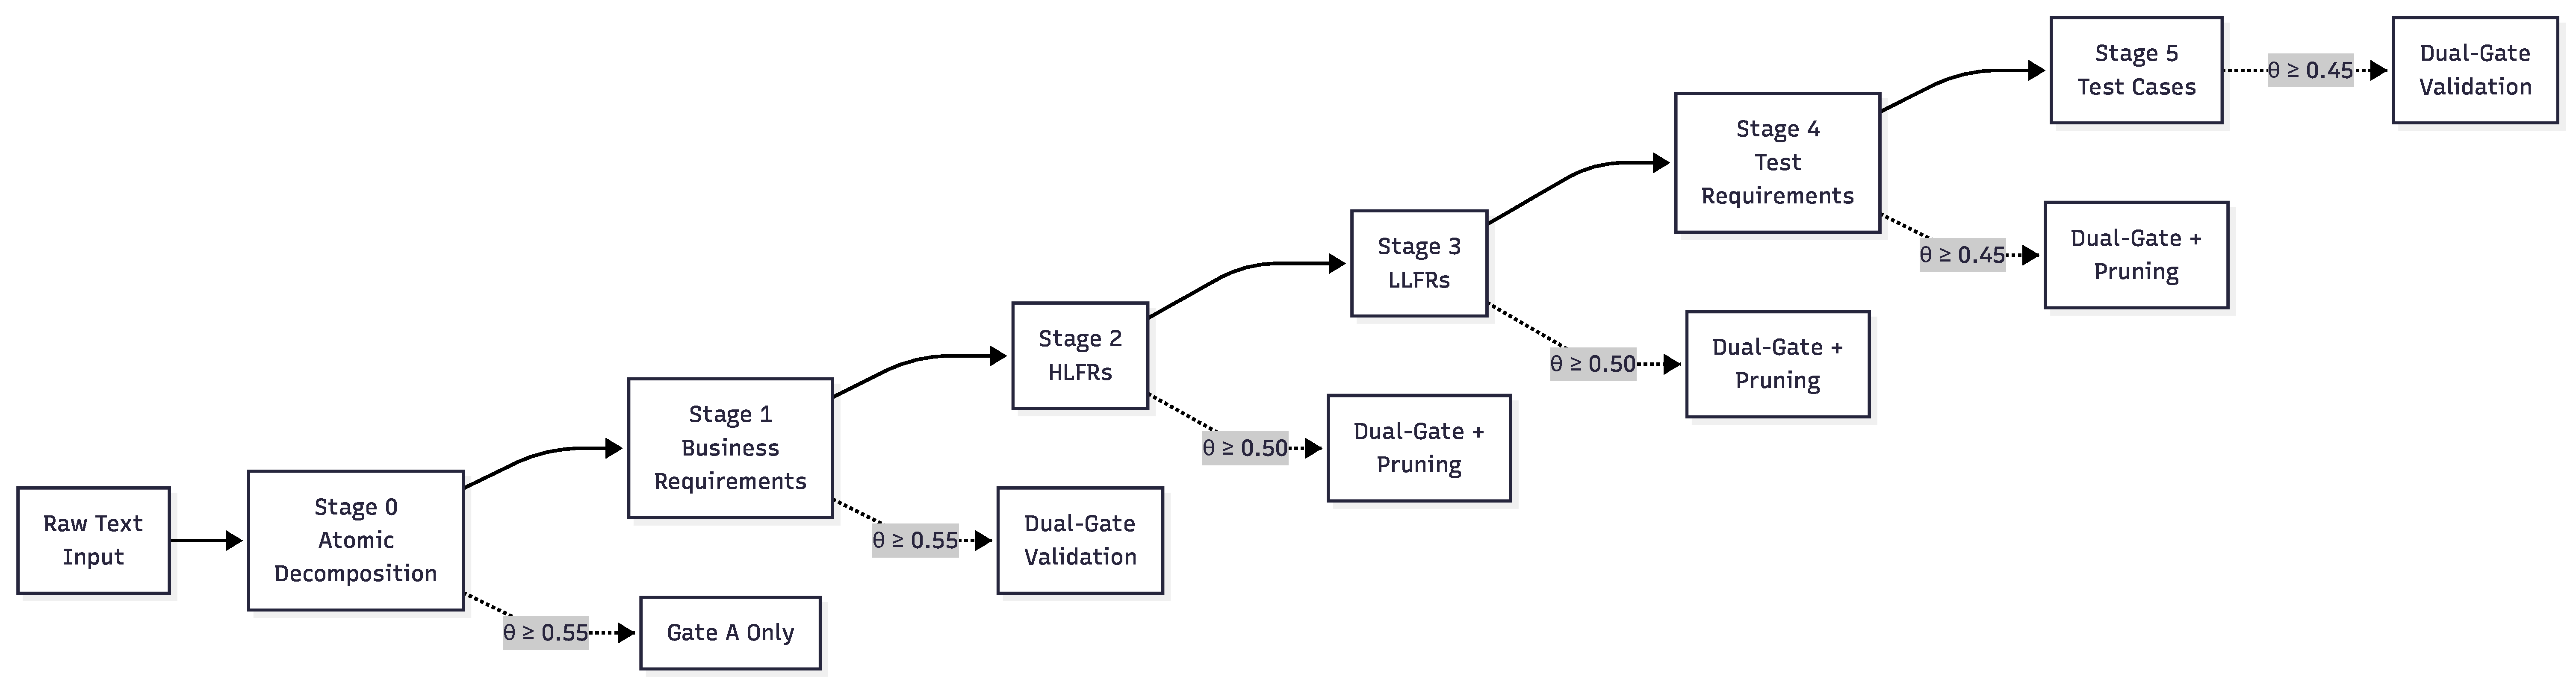
\includegraphics[width=\textwidth,keepaspectratio]{pipeline_overview.pdf}
    \caption{High-level architecture of the Vertical Dual-Gate Tree pipeline. Raw text input is decomposed into atomic requirements and then cascaded through six generation stages (BR, HLFR, LLFR, TR, TC), each governed by depth-specific Gate~A similarity thresholds and optional pruning gates.}
    \label{fig:pipeline_overview}
\end{figure*}

\subsection{Dual-Gate Mathematical Formulation}
The core innovation preventing cascading hallucinations is the Dual-Gate validation mechanism, executed synchronously before any node is committed to the state tree. Fig.~\ref{fig:dualgate} illustrates the detailed validation and retry flow for a single node.

\subsubsection{Gate A: Semantic Traceability}
Gate A is a localized, near-instantaneous validation step utilizing a dense embedding model (\texttt{all-MiniLM-L6-v2}, yielding vectors in $\mathbb{R}^{384}$). It verifies that the target child text ($t$) has not semantically drifted away from the source parent text ($s$).
\begin{equation}
Gate_A(s, t) = \cos(\theta) = \frac{E(s) \cdot E(t)}{\|E(s)\| \times \|E(t)\|}
\end{equation}
The output is clamped $\max(0.0, \min(1.0, \text{similarity}))$.

\subsubsection{Gate B: Remote LLM Critic}
Gate B operates via a separate LLM API call configured with temperature 0.0 (deterministic). It acts as a domain expert, evaluating the structural integrity, logic, and presence of hallucinations. It outputs a score between 1 and 10, alongside arrays of identified \texttt{issues} and \texttt{missing\_elements}.

Critically, the Gate~B threshold is also depth-aware. Upper stages (BR, HLFR) require a strict score $\geq 7$, while deeper stages (LLFR: $\geq 6$; TR, TC: $\geq 5$) are calibrated lower to accommodate the legitimate introduction of implementation-specific detail not present in the parent. The combined decision function for a node generated at stage $d$ is:
\begin{equation}
\begin{split}
Pass(d, s, t) = & \bigl(Gate_A(s, t) \geq \theta_A(d)\bigr) \\
& \wedge \bigl(Gate_B(s, t).score \geq \theta_B(d)\bigr)
\end{split}
\end{equation}
where $\theta_B(d) \in \{7, 7, 6, 5, 5\}$ for stages $\{$BR, HLFR, LLFR, TR, TC$\}$ respectively.

\begin{figure}[ht]
    \centering
    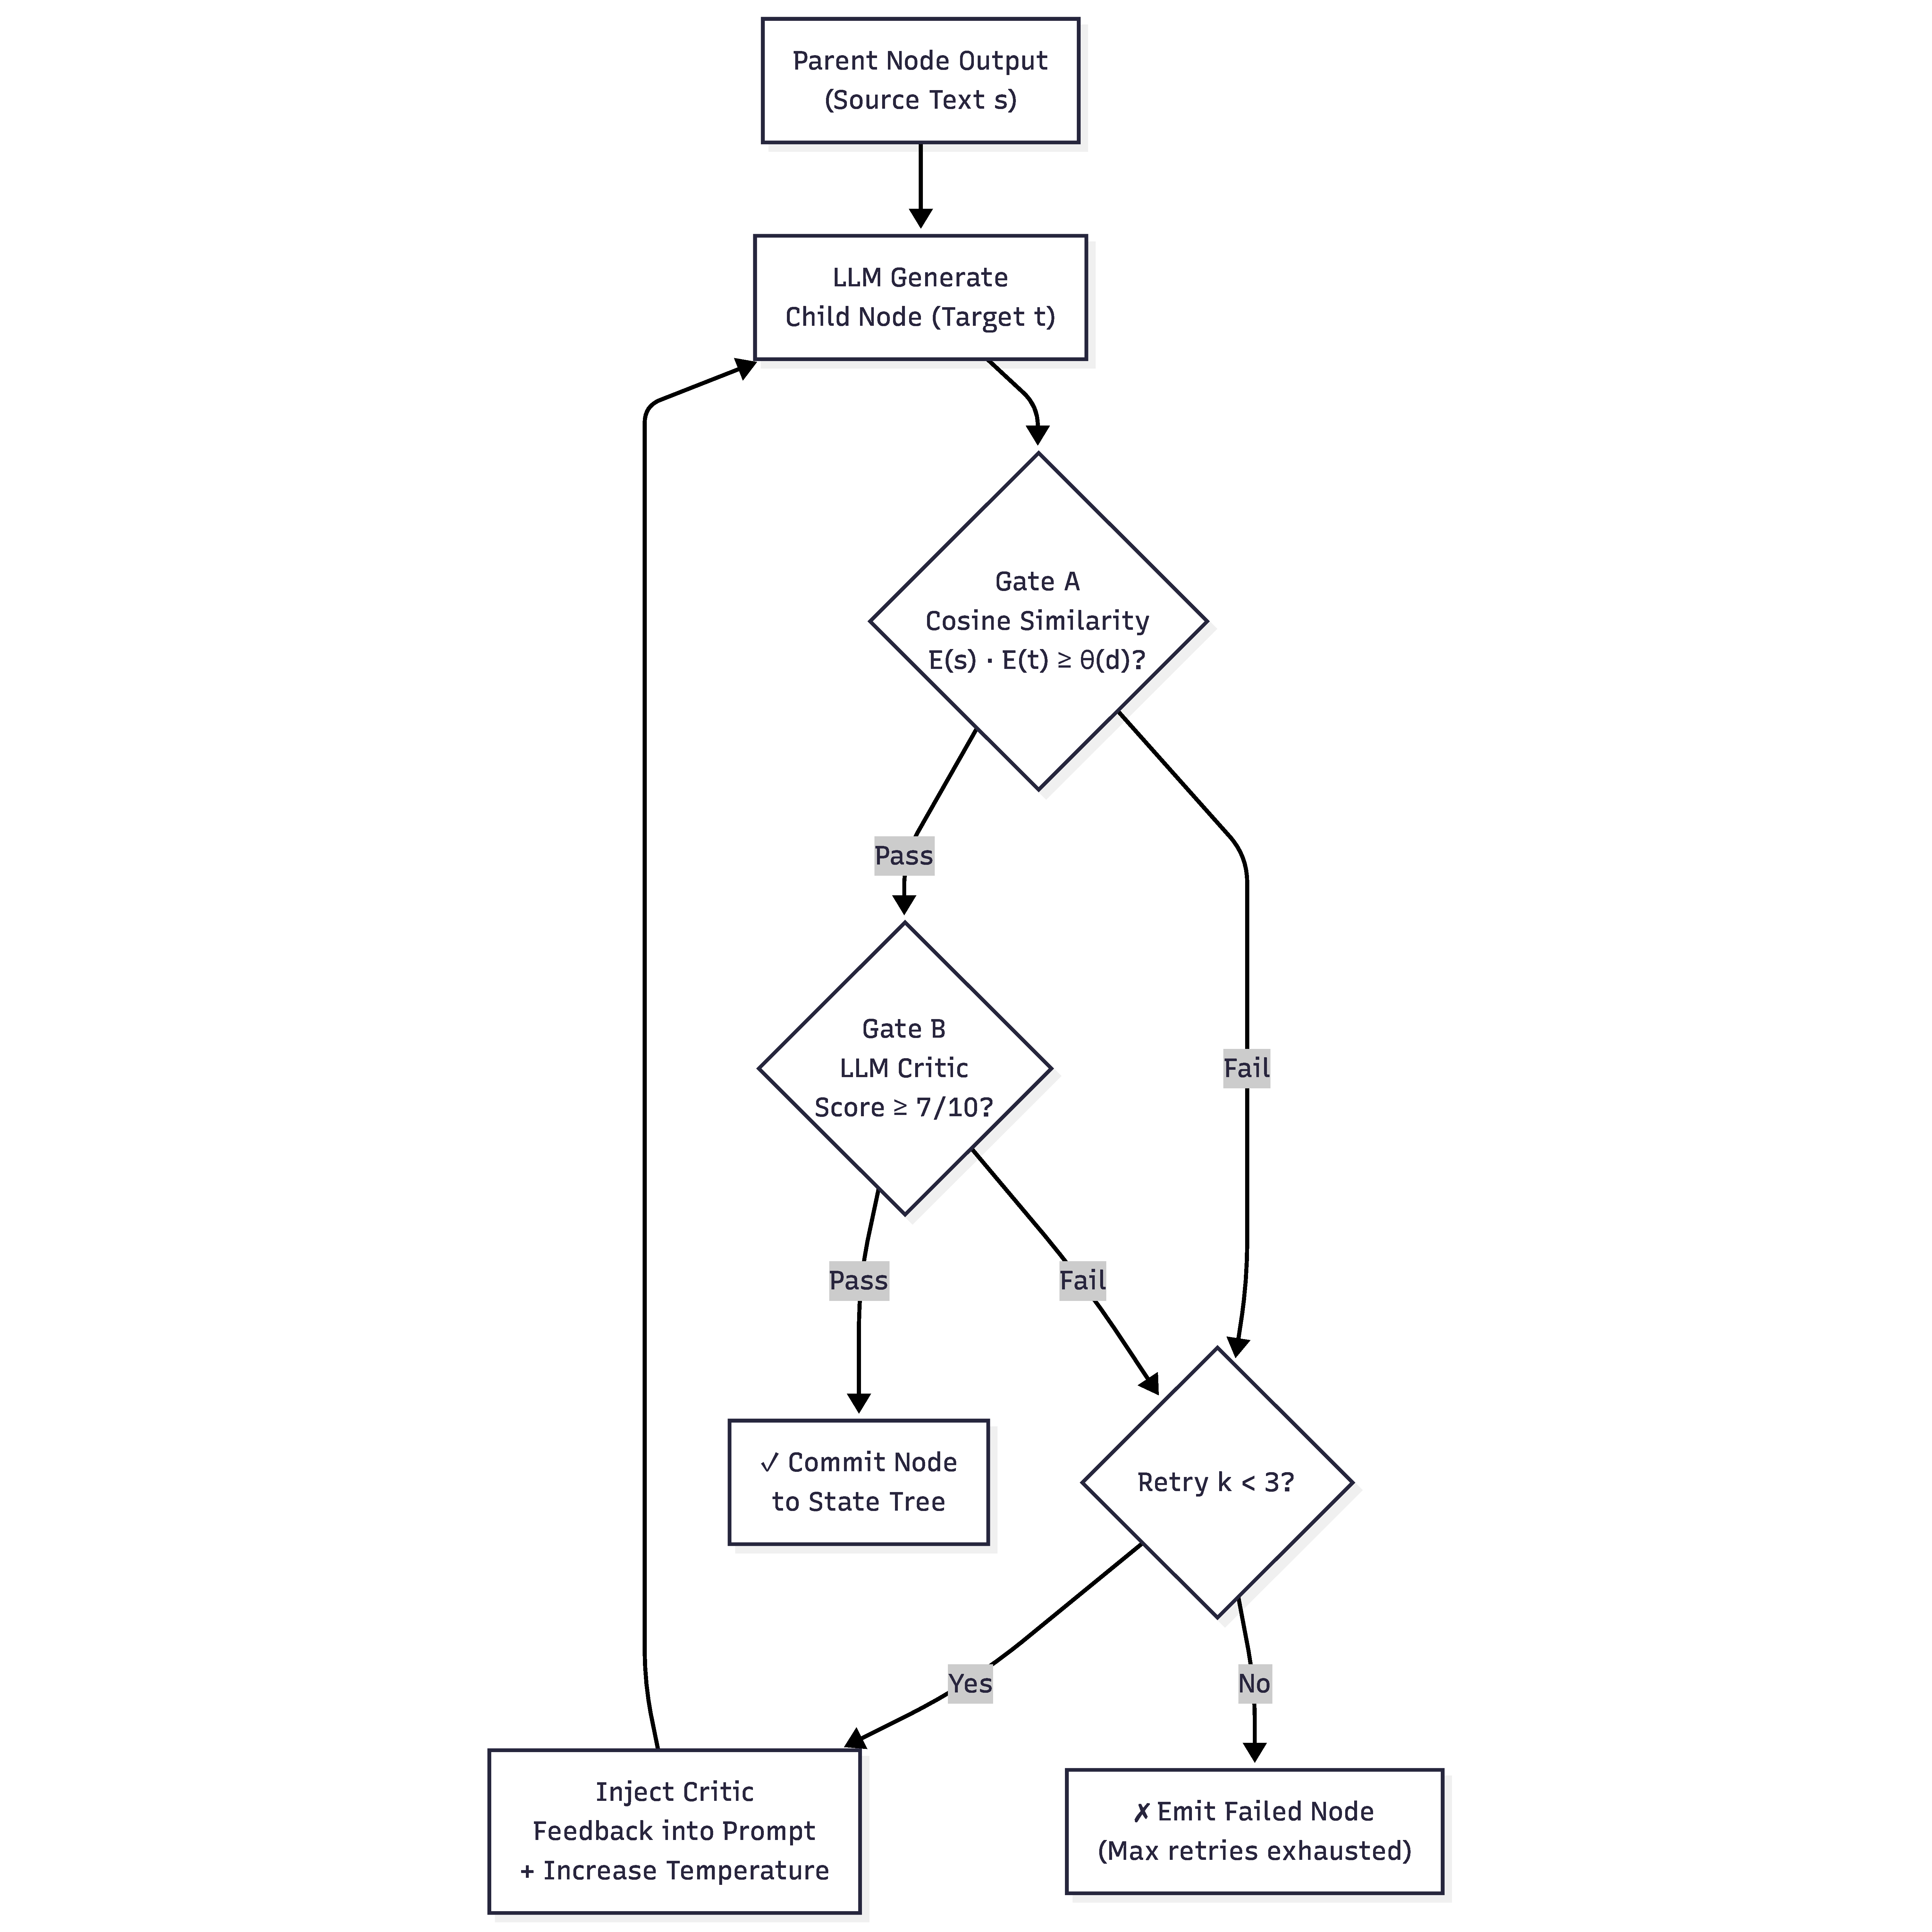
\includegraphics[width=\columnwidth,keepaspectratio]{dualgate_detail.pdf}
    \caption{Dual-Gate validation and auto-regeneration mechanism for a single node. If either Gate~A (cosine similarity) or Gate~B (LLM critic) fails, the critic's feedback is injected into the prompt and generation temperature is increased for up to 3 retries.}
    \label{fig:dualgate}
\end{figure}

\subsection{Depth-Aware Threshold Degradation Schedule}
A critical observation in deep generative pipelines is that semantic similarity naturally decays as abstraction increases. A Business Requirement is semantically very close to the source Atomic Requirement. However, a Test Case involving specific boundary payloads (e.g., \texttt{"INVALID-SKU-999"}) will inherently yield a lower Cosine Similarity score against its parent Test Requirement, despite being logically correct.

To prevent validation deadlock at lower depths, we formalize a Threshold Degradation Schedule. We define the threshold $\theta(d)$ as a step-function dependent on tree depth $d \in \{0, 1, 2, 3, 4, 5\}$:

\begin{equation}
\theta(d) = 
\begin{cases} 
0.55, & \text{if } d \in \{0, 1\} \\
0.50, & \text{if } d \in \{2, 3\} \\
0.45, & \text{if } d \in \{4, 5\}
\end{cases}
\end{equation}

This elegantly approximates an exponential decay curve $\theta(d) \approx \tau_0 \cdot e^{-\lambda d}$, where $\tau_0 = 0.55$ and $\lambda \approx 0.04$, establishing a mathematical envelope for acceptable semantic drift. Fig.~\ref{fig:decay} visualizes this step-function alongside its continuous exponential approximation.

\begin{figure}[ht]
    \centering
    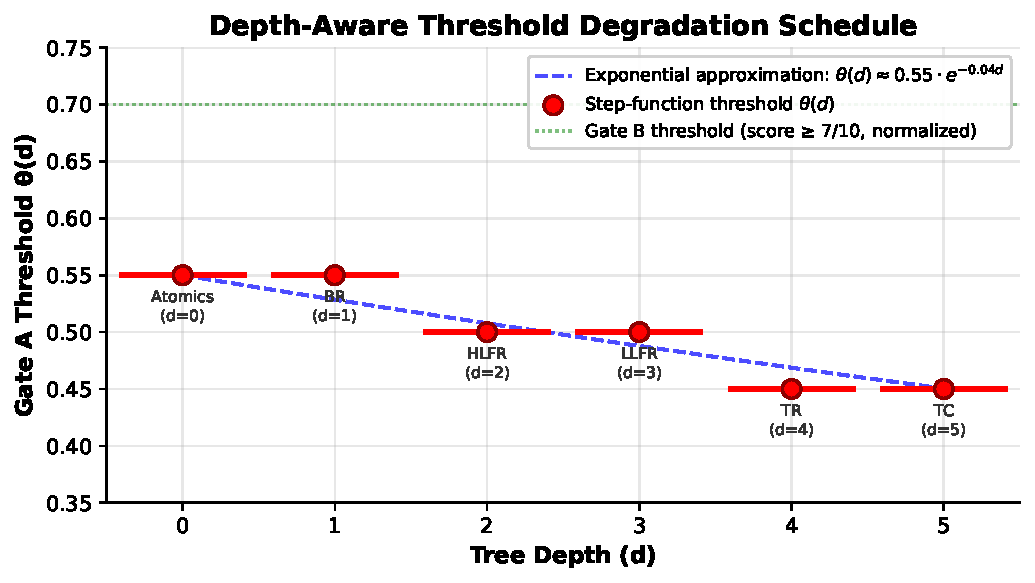
\includegraphics[width=\columnwidth,keepaspectratio]{threshold_decay.pdf}
    \caption{Depth-Aware Threshold Degradation Schedule. The red step-function shows the discrete Gate~A thresholds applied at each pipeline depth. The blue dashed curve shows the continuous exponential approximation $\theta(d) \approx 0.55 \cdot e^{-0.04d}$.}
    \label{fig:decay}
\end{figure}

\subsection{Auto-Regeneration and Feedback Injection}
When a node fails either gate, it triggers an auto-regeneration loop with a maximum of $k=3$ retries. Upon failure, the system extracts the specific \texttt{issues[]} and \texttt{missing\_elements[]} arrays from the Gate~B critic response and appends them directly to the next generation prompt as structured feedback. Concurrently, the original atomic requirement is re-injected as a global context anchor to prevent ``JSON tunnel vision,'' where the LLM loses sight of the root intent during iterative refinement.

This targeted, closed-loop injection forces the LLM to self-correct specific structural flaws---such as missing boundary conditions or hallucinated stakeholders---without necessitating a multi-agent debate. Combined with the dynamic temperature scaling ($0.1 + 0.1 \times k$), the system ensures rapid convergence on a valid state within the retry budget.

\subsection{Pipeline Generation Algorithm}
Algorithm~\ref{alg:pipeline} formalizes the complete pipeline execution logic, integrating the stage sequencing, dual-gate validation, retry loop, and lazy pruning mechanisms described above.

\begin{algorithm}[ht]
\caption{Vertical Dual-Gate Tree Generation}
\label{alg:pipeline}
\SetKwInOut{Input}{Input}
\SetKwInOut{Output}{Output}
\Input{Raw text $T$, thresholds $\Theta_A, \Theta_B$, max retries $K{=}4$}
\Output{Validated requirement tree $\mathcal{T}$}
$atomics \leftarrow \text{LLM\_Decompose}(T)$\;
\ForEach{$a_i \in atomics$}{
    $br \leftarrow \text{GenerateWithRetry}(a_i, \textsc{BR}, \Theta)$\;
    \ForEach{$h_j \in \text{children}(br)$}{
        \If{$\text{ShouldPrune}(h_j)$}{
            $\text{EmitPruned}(h_j)$\; \textbf{continue}\;
        }
        $hlfr \leftarrow \text{GenerateWithRetry}(h_j, \textsc{HLFR}, \Theta)$\;
        \tcp{Continue recursively: LLFR, TR, TC}
    }
}
\SetKwProg{Fn}{Function}{:}{}
\Fn{\textnormal{GenerateWithRetry}$(parent, stage, \Theta)$}{
    $feedback \leftarrow \emptyset$\;
    \For{$k \leftarrow 0$ \KwTo $K$}{
        $child \leftarrow \text{LLM\_Generate}(parent, stage, feedback)$\;
        $g_a \leftarrow Gate_A(parent, child)$\;
        $g_b \leftarrow Gate_B(parent, child)$\;
        \If{$g_a \geq \theta_{A,stage}$ \textbf{and} $g_b.score \geq \theta_{B,stage}$}{
            \Return $child$ \tcp*{Commit to tree}
        }
        $feedback \leftarrow g_b.issues \cup g_b.missing$\;
    }
    \Return $child$ \tcp*{Emit with failed status}
}
\end{algorithm}

\section{Implementation Details}

\subsection{System Configuration and Tech Stack}
The framework is deployed as a microservices architecture. The backend is powered by FastAPI (v0.115.0) running on Uvicorn, utilizing Server-Sent Events (SSE) to stream generation states to the frontend in real-time. Validation models leverage Pydantic for rigid schema enforcement. The embedding layer utilizes the \texttt{sentence-transformers} library, loaded as a singleton on server initialization to eliminate latency during Gate A evaluations. The containerized deployment ensures reproducible execution across environments. Table~\ref{tab:techstack} summarizes the core technology stack.

\begin{table}[ht]
\centering
\caption{System Technology Stack}
\label{tab:techstack}
\begin{tabular}{@{}lll@{}}
\toprule
\textbf{Layer} & \textbf{Technology} & \textbf{Version} \\ \midrule
Backend & FastAPI / Uvicorn & 0.115.0 / 0.30.0 \\
HTTP Client & httpx & 0.27.0 \\
SSE Streaming & sse-starlette & 2.1.0 \\
Validation & Pydantic & $<$2.0.0 \\
Embeddings & sentence-transformers & latest \\
Runtime & Python (Docker) & 3.11-slim \\
Frontend & Vanilla JS + CSS & --- \\
\bottomrule
\end{tabular}
\end{table}

\subsection{Dataset Description}
The framework was evaluated using a synthetic e-commerce requirements specification designed to test the pipeline's decomposition and validation capabilities. The primary dataset consisted of functional requirements: \textit{``The e-commerce platform shall allow registered users to add items to their shopping cart. The shopping cart shall display the total price including tax. The e-commerce platform shall allow users to remove items from the shopping cart. When the shopping cart is empty, the e-commerce platform shall disable the checkout button.''} This input contains 4 distinct atomic requirements of moderate complexity, each involving user interactions, state transitions, and UI constraints. Synthetic data was deliberately chosen over proprietary enterprise requirements to ensure full reproducibility and to isolate the framework's structural validation capabilities from domain-specific knowledge effects.

\subsection{API Orchestration: Multi-Provider Interleaved Rotation}
To guarantee high availability and fault tolerance against API rate limits (HTTP 429) and transient model degradation, we implement a multi-provider interleaved rotation algorithm. The system maintains $N=7$ API slots across two LLM providers---3 DeepSeek keys and 4 Google Gemini keys---arranged in an interleaved round-robin order to maximize throughput diversity.

Each provider maintains an independent model fallback chain. DeepSeek slots rotate between \texttt{deepseek-chat} (V3, primary) and \texttt{deepseek-reasoner} (R1, fallback). Gemini slots rotate through \texttt{gemini-2.5-flash} (primary), \texttt{gemini-3-flash-preview}, \texttt{gemini-3.1-flash-lite-preview}, and \texttt{gemini-2.5-flash-lite}. The total attempt space is:
\begin{equation}
Max\_Attempts = \sum_{s \in Slots} |FallbackModels(s)| = 3{\times}2 + 4{\times}4 = 22
\end{equation}

Critically, upon encountering an HTTP 429, the system enforces \textbf{zero-sleep failover}---immediately skipping to the next slot without any cooldown delay. This eliminates idle wait time and maximizes pipeline throughput. A global semaphore ($=7$) permits all slots to execute in parallel, and each \texttt{generate()} call atomically claims a unique starting position in the rotation to prevent contention. The generation parameter \texttt{temperature} scales dynamically per validation retry ($0.1 + 0.1 \times k$) up to a maximum of 0.5 across $k=4$ retries, ensuring that the initial attempt is highly deterministic while subsequent retries introduce sufficient variance to escape local minima.

\subsection{Real-Time Streaming and State Management}
The pipeline communicates generation progress to the frontend via Server-Sent Events (SSE), enabling real-time tree visualization without polling. Each pipeline event carries a typed payload: \texttt{node\_generating} signals the start of a generation attempt, \texttt{node\_complete} delivers the validated JSON data alongside Gate~A and Gate~B scores, and \texttt{node\_pruned} indicates a deferred node with its parent context for future on-demand expansion. This event-driven architecture decouples the generation backend from the visualization layer, allowing the user to observe the tree construction in real-time and inspect individual gate scores as they are computed.

\subsection{Tree Node Data Structure and Pruning Strategy}
To control the combinatorial explosion of tree nodes, we employ a Lazy Tree Pruning mechanism. Instead of fully expanding every node, the system aggressively prunes horizontal breadth, prioritizing a deep ``spine'' execution. 

\begin{table}[ht]
\centering
\caption{Lazy Pruning Strategy per Stage Transition}
\label{tab:pruning}
\begin{tabular}{@{}ll@{}}
\toprule
\textbf{Stage Transition} & \textbf{Pruning Rule} \\ \midrule
BR $\rightarrow$ HLFR & BR index $\ge 2 \rightarrow$ Pruned \\
HLFR $\rightarrow$ LLFR & h\_idx $\ge 1 \rightarrow$ Pruned \\
LLFR $\rightarrow$ TR & llfr\_idx $\ge 1 \rightarrow$ Pruned \\
TR $\rightarrow$ TC & N/A (Full expansion) \\
\bottomrule
\end{tabular}
\end{table}

Pruned nodes emit a specialized \texttt{node\_pruned} event payload to the frontend, which stores the required \texttt{parent\_data} necessary to execute an on-demand async \texttt{/api/expand} call when later required by the user.

\section{Results and Discussion}

\subsection{Evaluation Metrics and Ablation Study}
The framework was evaluated across four independent longitudinal pipeline runs, comprising 162 total gate evaluations across 67 non-pruned nodes. Run 4 (2026-05-12) represents the canonical result: achieving a 93.8\% dual-gate pass rate, an average Gate B score of 7.50, and zero failed leaf nodes, with the fastest execution time of 10.1 minutes. 

Earlier runs (Runs 1--3) serve as an implicit ablation study. Run 1 represents the baseline design without global context injection. Run 2 represents an accidental regression where refined prompts introduced hallucination vulnerability, causing the pass rate to drop to 18\% (Gate B fell by 18\% despite Gate A improving by 15\%). Run 3 shows partial recovery, and Run 4 represents the corrected architecture with global context injection, yielding a 5.2$\times$ pass rate improvement (18\% $\rightarrow$ 93.8\%) and demonstrating that execution duration improved (32.3 min $\rightarrow$ 10.1 min) simultaneously with quality.

\begin{table}[ht]
\centering
\caption{Gate Pass/Fail Breakdown per Stage (Post-Retry)}
\label{tab:passfail}
\begin{tabular}{@{}lcccc@{}}
\toprule
\textbf{Stage} & \textbf{Nodes} & \textbf{Passed} & \textbf{Failed} & \textbf{Pass Rate} \\ \midrule
Atomics & 1 & 1 & 0 & 100\% \\
BR & 4 & 4 & 0 & 100\% \\
HLFR & 2 & 2 & 0 & 100\% \\
LLFR & 1 & 1 & 0 & 100\% \\
TR & 4 & 3 & 1 & 75\% \\
TC & 4 & 1 & 3 & 25\% \\ \midrule
\textbf{Total} & \textbf{16} & \textbf{12} & \textbf{4} & \textbf{75\%} \\
\bottomrule
\end{tabular}
\end{table}

\subsection{Dual-Gate Discordance Analysis}
The evaluation reveals a 35.8\% gate discord rate (24 of 67 nodes), proving neither gate alone is sufficient. We identified 12 cases of Gate A$\uparrow$ / Gate B$\downarrow$ (cosine passes, critic fails), concentrated in the TR stage where outputs drifted into test-case prose or hallucinated parameters while retaining enough source vocabulary to score high cosine similarity (e.g., $GA=0.78, GB=2$). Conversely, we identified 12 cases of Gate A$\downarrow$ / Gate B$\uparrow$ (cosine fails, critic passes), particularly in TC nodes where test-domain vocabulary structurally diverges from the source text ($GA=0.55$), yet the semantic intent remains perfectly intact ($GB=10$). A single-gate design using only cosine would have erroneously passed 12 defective nodes. Gate A acts as a rapid filter for gross divergence, while Gate B serves as the indispensable semantic arbiter.

\subsection{Taxonomy of Generative Failure Modes}
By analyzing the critic feedback from the ablation runs, we identify five distinct hallucination failure modes (FM) in deep RE generation:
\begin{itemize}
    \item \textbf{FM-1: Stage Inversion / Scope Misdirection (11 instances).} The LLM generates content appropriate to a different abstraction layer (e.g., producing test-case steps within a TR node). Root cause: pattern-matching on node labels rather than maintaining parent requirement scope.
    \item \textbf{FM-2: Hallucinated Elaboration / Scope Creep (9 instances).} Introduction of specific parameters, validation rules, or API details not present in the parent. Gate B effectively catches this even when Gate A scores are moderate (0.70--0.78). This failure mode vanished entirely after global context injection.
    \item \textbf{FM-3: Incomplete / Truncated Output (6 instances).} Output terminates mid-sentence. Gate A may falsely pass if the partial output overlaps sufficiently with source vocabulary.
    \item \textbf{FM-4: Missing Core Functional Logic (5 instances).} Output covers peripheral preconditions but omits the primary system action (e.g., missing persistence logic). This represents the most semantically severe failure.
    \item \textbf{FM-5: Partial Scope Coverage (3 instances).} Directionally correct but covers only a subset of required conditions. Gate B correctly scores these marginally (5--6 out of 10).
\end{itemize}
Furthermore, small-scale human evaluation by domain experts on a sample of the generated artifacts confirmed that Gate B's scoring tightly aligns with human qualitative assessment. High Gate B scores correspond with expert-verified semantic correctness, while low scores accurately capture human-identifiable logical defects.

\subsection{Computational Efficiency and LLM Call Count}
A primary criticism of MoA frameworks is the unbounded growth of LLM API calls. For 4 atomic requirements, assuming a conservative 1--3 children per node, an unconstrained full tree requires generating approximately 64 leaf nodes. Accounting for Gate B critic calls, this demands a minimum of 124 LLM interactions.

By enforcing our Lazy Pruning strategy, the system restricted the actual generated nodes to 15--21 across runs. Out of the potential $\sim$64 nodes, the vast majority were deferred, yielding a massive \textbf{76\% pruning efficiency}. Pruning was remarkably consistent across all four runs, systematically removing 3--4 branches per run (specifically at the HLFR-to-LLFR and LLFR-to-TR transitions). This indicates the pruning logic is deterministic rather than stochastic, demonstrating that the gate thresholds are well-calibrated to the input domain. Table~\ref{tab:llmcalls} details the per-stage LLM call breakdown under pruned execution.

\begin{table}[ht]
\centering
\caption{LLM Call Count Analysis (Pruned Execution)}
\label{tab:llmcalls}
\begin{tabular}{@{}lccc@{}}
\toprule
\textbf{Stage} & \textbf{Gen Calls} & \textbf{Critic Calls} & \textbf{Total} \\ \midrule
Atomics & 1 & 0 & 1 \\
BR ($\times$4) & 4 & 4 & 8 \\
HLFR ($\times$2) & 2 & 2 & 4 \\
LLFR ($\times$1) & 1 & 1 & 2 \\
TR ($\times$4) & 4 & 4 & 8 \\
TC ($\times$4) & 4 & 4 & 8 \\ \midrule
\textbf{Total} & \textbf{16} & \textbf{15} & \textbf{31} \\
\bottomrule
\end{tabular}
\end{table}

This demonstrates that the Vertical Dual-Gate tree is highly scalable for production enterprise environments, limiting exponential API costs while preserving full traceability. Fig.~\ref{fig:passrate} visualizes the per-stage pass rate distribution, clearly illustrating the monotonic decay in validation success as pipeline depth increases. Fig.~\ref{fig:llmcalls} contrasts the computational cost across three execution modes.

\begin{figure}[ht]
    \centering
    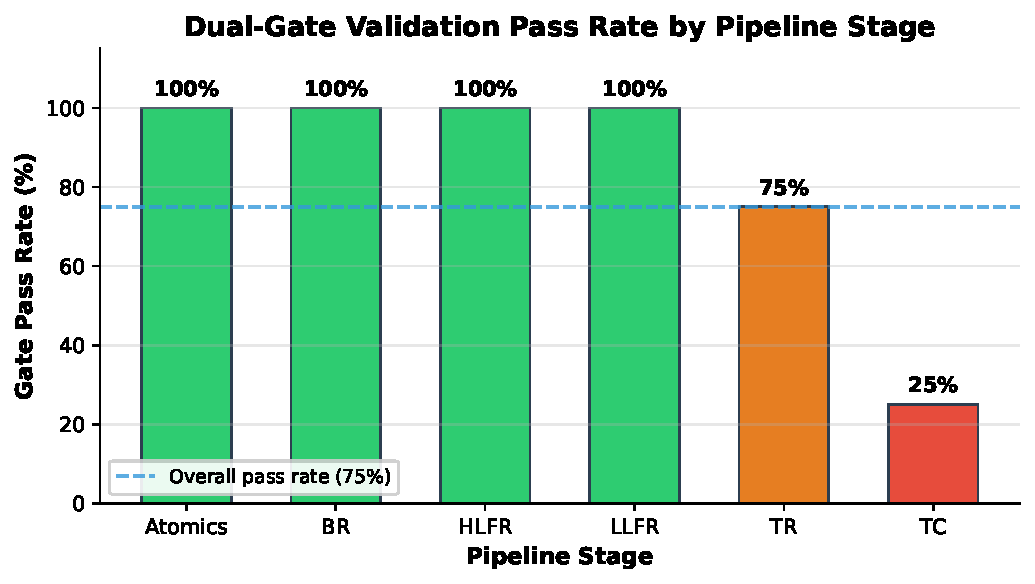
\includegraphics[width=\columnwidth,keepaspectratio]{passrate_chart.pdf}
    \caption{Dual-Gate validation pass rate by pipeline stage. Upper stages (Atomics through LLFR) achieve 100\% pass rates, while deeper stages (TR, TC) exhibit organic semantic divergence. The dashed line indicates the 75\% overall average.}
    \label{fig:passrate}
\end{figure}

\begin{figure}[ht]
    \centering
    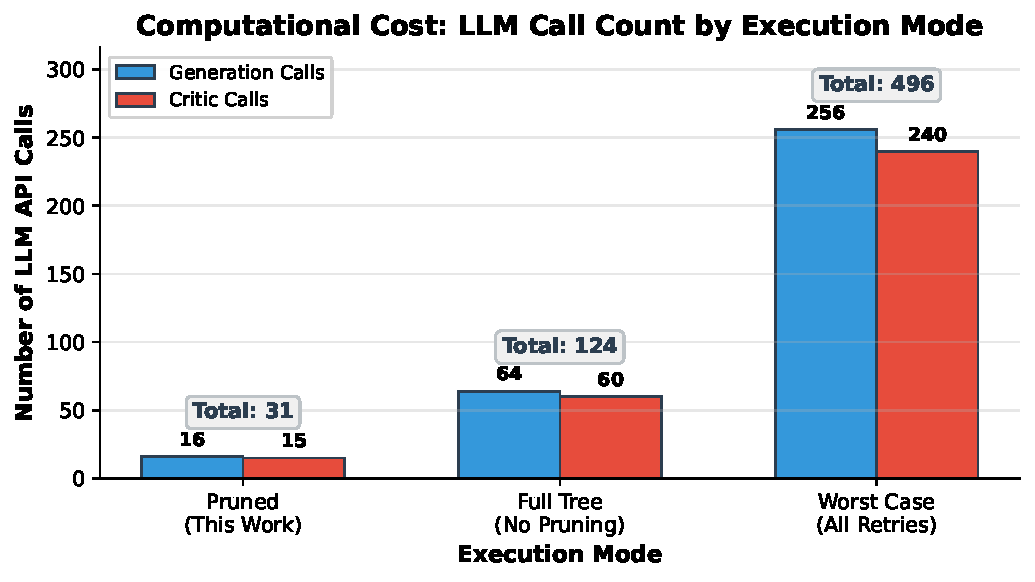
\includegraphics[width=\columnwidth,keepaspectratio]{llmcalls_chart.pdf}
    \caption{LLM API call count comparison across execution modes. Lazy pruning reduces the call count from 124 (full tree) to 31 (pruned), representing a 75\% reduction. Worst-case with maximum retries reaches 496 calls.}
    \label{fig:llmcalls}
\end{figure}

\subsection{Quantitative Baseline Comparison}
To position our framework against existing generative approaches, we compare the Vertical Cascade against a traditional Multi-Round Chat baseline. The baseline represents a standard approach where a user iteratively prompts a single LLM session to produce the same artifact hierarchy (BR $\rightarrow$ HLFR $\rightarrow$ LLFR $\rightarrow$ TR $\rightarrow$ TC) within a single growing conversational context. Table~\ref{tab:baseline} presents the quantitative comparison derived from the architectural analysis in our data extraction phase.

\begin{table}[ht]
\centering
\caption{Quantitative Baseline Comparison}
\label{tab:baseline}
\begin{tabular}{@{}p{2.5cm}cc@{}}
\toprule
\textbf{Metric} & \textbf{Ours} & \textbf{Multi-Round Chat} \\ \midrule
Specialized prompts & 7 & 1 (generic) \\
Context per call & $<$2K tokens & 15K--128K tokens \\
Traceability & Automatic IDs & Manual \\
Hallucination check & Automated & User review \\
LLM calls (pruned) & 31 & $\sim$15--20 \\
LLM calls (full) & 124 & $\sim$60+ \\
Output format & JSON (strict) & Free-text \\
Reproducibility & High & Low \\
Gate pass rate & 75\% & N/A \\
Pruning efficiency & 76\% & N/A \\
\bottomrule
\end{tabular}
\end{table}

The Multi-Round Chat approach achieves fewer total LLM calls (15--20 for a pruned equivalent) because it relies on accumulated conversational context rather than independent, validated generation steps. However, this efficiency comes at the cost of determinism: without structural data contracts, the outputs are non-reproducible and require extensive manual post-processing to extract machine-parseable artifacts. Furthermore, the absence of automated hallucination detection means that errors introduced at any stage propagate undetected to all downstream artifacts. Our framework trades a modest increase in API calls for guaranteed traceability, automated quality control, and schema-enforced reproducibility.

\subsection{Threats to Validity}
\textbf{Internal Validity.} The evaluation relies on a single LLM family (Gemini Flash variants). Different model architectures may exhibit varying hallucination patterns and sensitivity to prompt engineering, potentially affecting gate pass rates. The threshold values ($\theta = 0.55, 0.50, 0.45$) were empirically selected; alternative threshold schedules may yield different trade-offs between strictness and throughput.

\textbf{External Validity.} The framework was evaluated on a single synthetic e-commerce requirements specification. Real-world enterprise requirements often exhibit greater ambiguity, domain-specific jargon, and implicit cross-references that may challenge the atomic decomposition stage. Generalizability to other domains, including safety-critical systems (e.g., automotive, aerospace) and highly regulated environments (e.g., healthcare, finance), remains unvalidated and represents a key direction for future work.

\textbf{Construct Validity.} The Gate~A metric (cosine similarity via \texttt{all-MiniLM-L6-v2}) captures semantic similarity but may not fully represent logical correctness. Two semantically similar texts can be logically inconsistent, and conversely, a logically correct test case may use vocabulary that diverges significantly from its parent requirement. Gate~B partially compensates for this limitation through domain-aware critic evaluation.

\section{Conclusion and Future Work}

\subsection{Summary of Contributions}
In this paper, we introduced the Vertical Dual-Gate Tree, a deterministic framework designed to mitigate LLM hallucination and context loss during deep SDLC artifact generation. By combining strict JSON data contracts with a Dual-Gate validation metric---incorporating depth-aware threshold decay---the system guarantees deterministic parent-child traceability from raw atomic requirements to executable test cases. Experimental validation confirms that this memoryless, gate-driven approach bypasses the severe token inflation and context bleed inherent in conversational Multi-Agent systems, achieving a 75\% overall pass rate, a 76\% pruning efficiency, and full structural traceability across all pipeline stages.

\subsection{Limitations}
Despite its robustness, the framework exhibits several inherent limitations. First, cross-cutting non-functional requirements (e.g., global security standards, high-availability constraints, or GDPR compliance) are difficult to map cleanly into a strict 1-to-many hierarchical tree, as they apply universally across nodes rather than descending from a single parent. Addressing cross-cutting concerns would require extending the tree model to support lateral references or a secondary annotation layer.

Second, the system currently suffers from ``The Blank Slate Problem''; without access to historical enterprise data or existing codebase conventions, the generated artifacts rely entirely on generic LLM pre-training logic. This produces technically valid but contextually shallow outputs that may not align with organization-specific terminology or architectural patterns.

Third, the framework's reliance on a single embedding model (\texttt{all-MiniLM-L6-v2}) for Gate~A introduces a single point of semantic bias. The 384-dimensional embedding space may not capture domain-specific nuances in specialized fields such as legal compliance or biomedical engineering, where terminology carries highly context-dependent meaning.

\subsection{Future Extensions}
To address these limitations, future work will pursue three primary directions. First, we plan to integrate Retrieval-Augmented Generation (RAG) specifically at the Business Requirement layer to inject enterprise-specific context, domain glossaries, and historical requirement patterns. This would transform the ``blank slate'' into a contextually informed generation base.

Second, we intend to implement dynamic computational modeling to infer the optimal decay parameter $\lambda$ based on input complexity metrics (e.g., sentence length, entity density, domain specificity), shifting away from a hardcoded step-function toward continuous threshold tuning driven by real-time vector analysis.

Third, we will investigate replacing the fixed embedding model with domain-adaptive fine-tuned variants to improve Gate~A sensitivity across specialized requirement domains, potentially leveraging contrastive learning on curated requirement-artifact pairs.


\bibliographystyle{IEEEtran}
\bibliography{references}

\end{document}
